\documentclass[12pt]{article}
\usepackage[utf8]{inputenc}
\usepackage{float}
\usepackage{amsmath}

\usepackage{tikz}
\usepackage[hmargin=3cm,vmargin=6.0cm]{geometry}
\topmargin=-2cm
\addtolength{\textheight}{6.5cm}
\addtolength{\textwidth}{2.0cm}
\setlength{\oddsidemargin}{0.0cm}
\setlength{\evensidemargin}{0.0cm}
\usepackage{indentfirst}
\usepackage{amsfonts}

\usepackage{listings}

\begin{document}

\section*{Student Information}

Name : Ömer Kılınç\\

ID : 2448603\\


\section*{Answer 1}

\begin{equation}
f_{X,Y}(x,y) =
    \begin{cases}
        x+ky^3 & 0 \leq x \leq 1 \text{ , } 0 \leq y \leq 1 \\
        0 & 0 \text{ otherwise}
    \end{cases}
\end{equation}


\subsection*{a)} 

\[\textbf{By the definition of probability density function: }\]
\[\int_{-\infty}^{\infty}\int_{-\infty}^{\infty}f_{X,Y}(x,y) dx dy = 1\]
\[\]
\[\int_{-\infty}^{\infty}\int_{-\infty}^{\infty}x+ky^3 dx dy = 1\]

\[ = \int_{0}^{1}\int_{0}^{1}x+ky^3 dx dy\]

\[ = \int_{0}^{1}(\frac{x^2}{2}+kxy^3 \Big|_0^1)dy \]

\[ = \int_{0}^{1}\frac{1}{2}+ ky^3 dy \]

\[ = \frac{x^2}{2}y+ k\frac{y^4}{4} \Big|_0^1 \]

\[ = \frac{1}{2} + \frac{k}{4} = 1 \]

\[ k = 2\]

\subsection*{b)} 

\[P(X = x) = \int_{x}^{x}f_X(\tau) d\tau = 0\]
\[ \textbf{X has continuous distribution.} \]
\[ \textbf{Probability of X having a particular value is zero for any X = x} \]

\[P(X = x) = 0 \]


\subsection*{c)} 

\[\textbf{Computing the probability of Joint Distribution: }\]
\[P((X,Y) \in A) = \int\int_{(x,y)\in A}f_{X,Y}(x,y) dx dy \]

\[ P( 0 \leq x \leq 1 , 0 \leq y \leq 1 ) = \int_{0}^{1/2}\int_{0}^{1/2}x+2y^3 dx dy \]

\[ = \int_{0}^{1/2}(\frac{x^2}{2}+2xy^3 \Big|_0^{1/2})dy \]

\[ = \int_{0}^{1/2}\frac{1}{8}+y^3 dy \]

\[ = (\frac{1}{8}y + \frac{y^4}{4}) \Big|_0^{1/2} \]

\[ = 1/16 + 1/64 = \frac{5}{64}\]


\[ P( 0 \leq x \leq 1 , 0 \leq y \leq 1 ) = \frac{5}{64} \]


\section*{Answer 2}

\[f_{X,Y}(x,y) = \frac{e^{ -y-\frac{x}{y} } } {y}  \text{   for } 0 < x,y < \infty\]


\subsection*{a)} 

\[f_Y(y) = \int_{-\infty}^{\infty} f_{X,Y}(x,y) dx \]

\[ = \int_{0}^{\infty} \frac{e^{ -y-\frac{x}{y} } } {y} dx  \]

\[ = \frac{e^{-y}}{y} \int_0^{\infty} e^{-\frac{x}{y} } dx \]

\[\textbf{Solving the integral part: }  \]

\[u = -\frac{x}{y}\]
\[ du = -\frac{1}{y}dx\]
\[ -y du = dx\]

\[ \int_0^{\infty} e^{-\frac{x}{y}} dx =  -y\int_0^{-\infty} e^u du = -y(e^u \big|_0^{-\infty}) = y\]


\[ \textbf{Inserting the result to equation:} \]
\[f_Y(y) = \frac{e^{-y}}{y}y = e^{-y} \]

\[f_Y(y) = e^{-y} \textbf{ for }x > 0 \]
\[ \textbf{Y has exponential distribution with } \lambda = 1\]


\subsection*{b)} 

\[f_Y(y) = e^{-y} \textbf{ for }x > 0 \]

\[E(Y) = \int_{-\infty}^{\infty} yf_Y(y) dy  =  \int_{0}^{\infty} ye^{-y} dy \]

\[ u = y \Longrightarrow  du = dy \]
\[ dv = e^{-y}dy \Longrightarrow  v = -e^{-y} \]

\[\int_{0}^{\infty} ye^{-y} dy = -e^{-y}y \big|_0^{\infty} - 
\int_0^{\infty} -e^{-y} dy \]

\[ = 0 + \int_0^{\infty} e^{-y}dy \]

\[-e^{-y} \big|_0^{\infty} = 0 - (-1) = 1\]

\[E(Y) = 1\]

\section*{Answer 3}

\[\textbf{p : probability that a soldier is naval.}\]
\[p = 0.1\]

\[\textbf{X : Number of navals in a randomly selected group of n soldiers.}\]
\[\textbf{X has binomial distribution since a soldier is either naval or not with p = 0.1 and n }\]


\subsection*{a)} 

\[ n = 1000 \text{ and } p = 0.1\]
\[ P(X \geq 1000(0.09) ) = P(X \geq 90 ) = 1 - P( X < 90) \]

\[\textbf{Using the Normal approximation to Binomial Distribution}\]
\[ \textbf{in order to calculate } P(X < 90)\]

\[ Binomial(n,p) \approx Normal(\mu,\sigma)\]

\[ P(X \geq 90) = 1 - P(X < 90))\]

\[ \mu = np = 100 \textbf{ and } \sigma = \sqrt{np(1-p)} = \sqrt{90} = 0.487\]

\[P(X<90) = P(X<89.5) \]
\[\text{Since X is strictly less than 90, equality holds}\]


\[P(X<89.5) = P(\frac{X-100}{0.487} < \frac{89.5-100}{9.487}) \]
\[ = \Phi(-1.10) = 0.1357\]

\[ 1 - P(X<90) = 1 - 0.1357 \]
\[= 0.8643 \]



\subsection*{b)} 
\[\textbf{Similarly, n=2000 and p = 0.1}\]
\[ Binomial(n,p) \approx Normal(\mu,\sigma)\]

\[ \mu = np = 200 \textbf{ and } \sigma = \sqrt{np(1-p)} = \sqrt{180} = 13.416\]

\[ P(X \geq 200 ) = P(X \geq 180 ) = 1 - P( X < 180) \]

\[P(X<180) = P(X<179.5) \]

\[= P(\frac{X-200}{13.416} < \frac{179.5-200}{13.416}) \]

\[ = \Phi(-1.52) = 0.0643\]

\[P(X \geq 180) = 1 - 0.0643 = 0.9357 \]

\[\textbf{Increasing the sample size makes the distribution get closer}\]
\[\textbf{to Normal Distribution (Cental Limit Theorem) }\]


\section*{Answer 4}

\[\textbf{T : Lifespan of an elephant in years.}\]
\[\textbf{T has normal distribution with: }\]
\[ \mu = 65 \text{ years and } \sigma = 6 \text{ years}\]

\subsection*{a)}

\[ P(60<T<75) \]
\[ \textbf{Converting from Normal to Uniform Normal:} \]

\[ P(\frac{60-65}{6} < \frac{T-65}{6} < \frac{75-65}{6}) \]

\[ = P(-0.83 < Z < 1.66) \]

\[ = \Phi(1.66) - \Phi(-0.83) \]
\[ = 1 - \Phi(-1.66) - \Phi(-0.83) \]
\[= 1 - 0.0485 - 0.2061 \]
\[= 0.7454 \]

\subsection*{b)} 

\begin{lstlisting}
u = 65;
q = 6;

N = [20, 100, 1000];

for i = 1:3

    sample = normrnd(u, q, N(i), 1);
    
    figure;
    
    hist(sample, 25);
    
    xlabel('Lifespan (years)');
    ylabel('Frequency');
    
end
\end{lstlisting}

\begin{figure}
  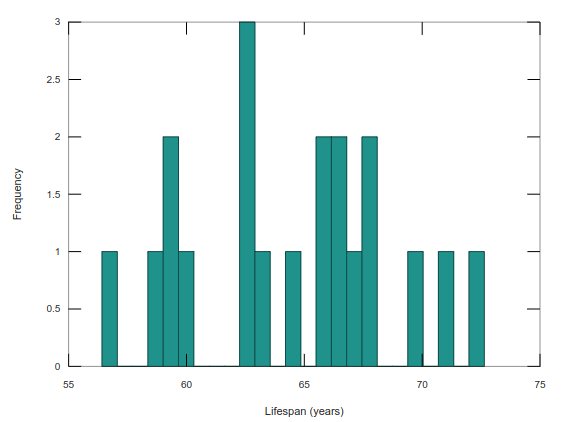
\includegraphics[width=\linewidth]{4b_N=20.png}
  \label{N=20}
  \caption{N=20}
\end{figure}

\begin{figure}
  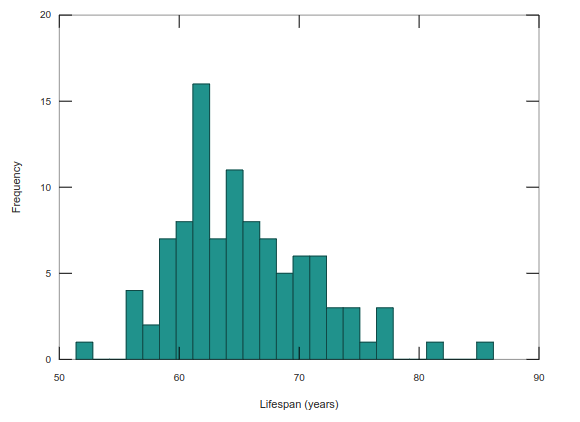
\includegraphics[width=\linewidth]{4b_N=100.png}
  \label{N=100}
  \caption{N=100}
\end{figure}

\begin{figure}
  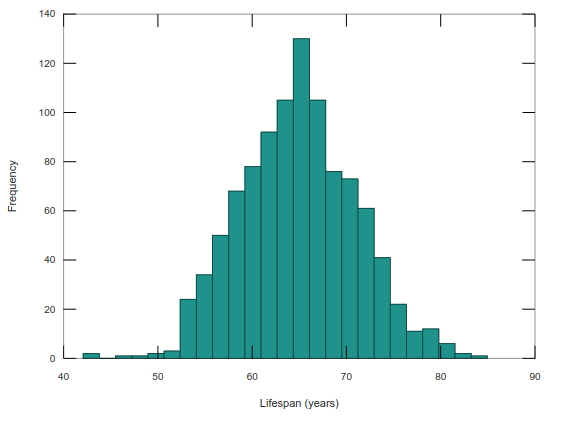
\includegraphics[width=\linewidth]{4b_N=1000.png}
  \label{N=1000}
  \caption{N=1000}
\end{figure}




\end{document}
